\section{Three attempts to improve the E4B baseline}\label{sec:programmes}

With a runner that could be trusted and a baseline that repeats, we tried three times to raise E4B's solved share.
The three programmes changed different things. The first changed the prompt; one of its variants changed a
thinking-token limit instead. The second changed the way the agent edits files. The third added a sub-agent step. What
exactly was changed is withheld with the bundle until the end of the competition (\cref{sec:setting}); the arms are
named in \cref{tab:arms}, and every run is in \texttt{runs.csv}.

Each programme followed the same four steps.
\begin{enumerate}[leftmargin=*,itemsep=1pt,topsep=2pt]
\item \emph{Build} several variants of the baseline bundle.
\item \emph{Pilot} (programmes 2 and 3 only): run first builds on 15 or 16 tasks, one run each, to find defects.
\item \emph{Screen}: run the variants and the unchanged baseline in one job queue on the 48 tasks of S, two repeats
each, and take the variant with the most solved runs as the candidate.
\item \emph{Confirm}: register the candidate, the tasks, the rule and the analysis script, then run candidate and
baseline once on a frozen panel that shares no task with S, and apply the pass rule of \cref{sec:compare}.
\end{enumerate}
The whole sequence for one programme took 1,152 to 1,402 runs and three to five hours of workstation time.

\subsection{Pilots and screens}\label{sec:screens}

\begin{table}[p]
\centering
\footnotesize
\caption{Pilot, development and screen blocks of the E4B candidates on the workstation. Lead: difference to the baseline of the same block in percentage points. Agent: mean seconds of the agent phase.}
\label{tab:screens}
\begin{tabular}{llrrrrrr}
\toprule
Block & Arm & Tasks & Runs & Solved & \% & Lead & Agent \\
\midrule
\texttt{pilot-2a} & \texttt{v-t1} & 15 & 15 & 4 & 26.7 & --- & 98 \\
\texttt{pilot-2a} & \texttt{v-t2} & 15 & 15 & 5 & 33.3 & --- & 71 \\
\addlinespace
\texttt{pilot-2b} & \texttt{v-t3} & 15 & 15 & 3 & 20.0 & --- & 96 \\
\texttt{pilot-2b} & \texttt{v-t4} & 15 & 15 & 7 & 46.7 & --- & 89 \\
\texttt{pilot-2b} & \texttt{v-t5} & 15 & 15 & 6 & 40.0 & --- & 77 \\
\texttt{pilot-2b} & \texttt{v-t6} & 15 & 15 & 6 & 40.0 & --- & 66 \\
\addlinespace
\texttt{dev-3} & \texttt{base} & 16 & 16 & 4 & 25.0 & --- & 58 \\
\texttt{dev-3} & \texttt{v-a1} & 16 & 16 & 2 & 12.5 & \ensuremath{-}12.5 & 48 \\
\texttt{dev-3} & \texttt{v-a2} & 16 & 16 & 3 & 18.8 & \ensuremath{-}6.2 & 54 \\
\addlinespace
\texttt{screen-1} & \texttt{base} & 48 & 96 & 19 & 19.8 & --- & 64 \\
\texttt{screen-1} & \texttt{v-b1} & 48 & 96 & 22 & 22.9 & +3.1 & 72 \\
\texttt{screen-1} & \texttt{v-p1} & 48 & 96 & 24 & 25.0 & +5.2 & 64 \\
\texttt{screen-1} & \texttt{v-p2} & 48 & 96 & 25 & 26.0 & +6.2 & 75 \\
\texttt{screen-1} & \texttt{v-p3} & 48 & 96 & 22 & 22.9 & +3.1 & 63 \\
\texttt{screen-1} & \texttt{v-p4} & 48 & 96 & 24 & 25.0 & +5.2 & 77 \\
\addlinespace
\texttt{screen-2} & \texttt{base} & 48 & 96 & 21 & 21.9 & --- & 72 \\
\texttt{screen-2} & \texttt{v-t4} & 48 & 96 & 18 & 18.8 & \ensuremath{-}3.1 & 88 \\
\texttt{screen-2} & \texttt{v-t6} & 48 & 96 & 22 & 22.9 & +1.0 & 89 \\
\addlinespace
\texttt{screen-3} & \texttt{base} & 48 & 96 & 20 & 20.8 & --- & 66 \\
\texttt{screen-3} & \texttt{v-a3} & 48 & 96 & 25 & 26.0 & +5.2 & 77 \\
\texttt{screen-3} & \texttt{v-a4} & 48 & 96 & 19 & 19.8 & \ensuremath{-}1.0 & 77 \\
\bottomrule
\end{tabular}
\end{table}


\Cref{tab:screens} lists every pilot and screen block.

\paragraph{Pilots.}
Programme 2 began with two first builds on 15 tasks of the case-study panel (\texttt{pilot-2a}), which solved 4 and
5 of 15, and continued with four rebuilds on the same tasks (\texttt{pilot-2b}), which solved 3, 7, 6 and 6. No
baseline ran in these two blocks. Of the four rebuilds, \arm{v-t4} and \arm{v-t6} went on to the screen. Programme 3
began with two first builds on 16 tasks of the small panel C (\texttt{dev-3}); they solved 2 and 3 of 16 against 4
for the baseline in the same queue, and both were rebuilt before the screen. The 16 tasks of \texttt{dev-3} belong to
the panel of the first confirmation, which had ended by then, and to no later one.

The pilots were meant to find builds that did not work. They ranked nothing. \arm{v-t4} had the best pilot
result, 7 of 15, and then solved fewer runs than the baseline in its screen.

\paragraph{Screens.}
In the first screen all five variants solved more runs than the baseline, 22 to 25 of 96 against 19, and the leader,
\arm{v-p2}, led by $\LeadOne$ points. In the second screen, \arm{v-t6} led by $\LeadTwo$ points and \arm{v-t4}
trailed. In the third, \arm{v-a3} led by $\LeadThree$ points and \arm{v-a4} trailed. All three leaders used more
agent time than the baseline of their screen: 75 against 64~s, 89 against 72~s and 77 against 66~s.

\subsection{Confirmation runs}\label{sec:confirm}

\begin{figure}[t]
\centering
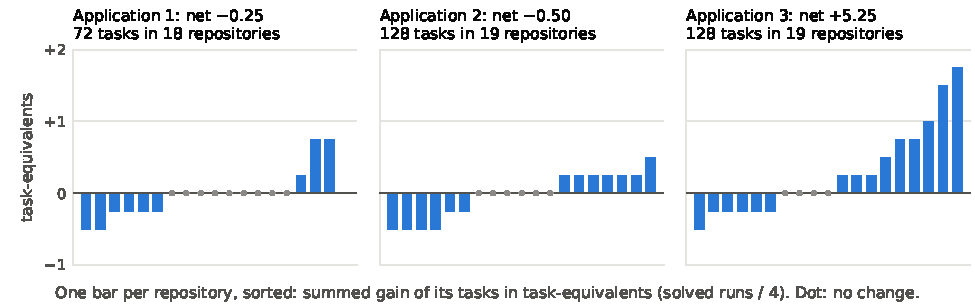
\includegraphics[width=\linewidth]{fig/supp_gates.pdf}
\caption{Gain of each repository in the three applications of the pass rule (candidate minus baseline). Repositories
are sorted by their total within each application.}
\label{fig:s-gates}
\end{figure}

\begin{table}[!htb]
\centering
\caption{Every application of the pass rule of \cref{sec:compare} to a real candidate, from the frozen gate reports. Baseline and candidate are two versions of the withheld agent bundle.}\label{tab:s-gates}
\footnotesize
\begin{tabular}{lrrr}
\toprule
 & Application 1 & Application 2 & Application 3 \\
\midrule
Task set & small panel & large panel minus small & as application 2 \\
Tasks; repositories; repeats & 72; 18; 4 & 128; 19; 4 & 128; 19; 4 \\
Runs per arm (all with a result row) & 288 & 512 & 512 \\
Solved runs: baseline, candidate & 63, 62 & 103, 101 & 97, 118 \\
Mean gain (points; exact fraction) & ${-}0.35$ (${-}1/288$) & ${-}0.39$ (${-}1/256$) & ${+}4.10$ ($21/512$) \\
\quad (1) gain at least $2/58$ & not met & not met & met \\
Bootstrap-$t$; one-sided $p$ (9{,}999 draws) & ${-}0.175$; 0.6034 & ${-}0.366$; 0.6034 & ${+}1.954$; 0.0405 \\
One-sided $p$ by exact enumeration & 0.6113 & 0.6067 & 0.0360 \\
\quad (2) $p \le 0.025$ & not met & not met & not met \\
Repositories gaining; losing & 3; 6 & 7; 6 & 9; 6 \\
\quad (3a) at least three repositories gain & met & met & met \\
Lowest leave-one-repository-out gain (points) & ${-}1.47$ & ${-}0.85$ & ${+}2.94$ \\
\quad (3b) every leave-one-out gain positive & not met & not met & met \\
Agent time, candidate / baseline (s) & 68.4 / 66.6 & 89.3 / 75.6 & 79.4 / 72.0 \\
\quad (4a) ratio at most 1.2 & 1.026: met & 1.182: met & 1.103: met \\
Infrastructure rows: baseline, candidate & 0, 0 & 0, 0 & 0, 0 \\
\quad (4b) infrastructure errors do not rise & met & met & met \\
Worst repository total (task-equivalents) & ${-}0.50$ & ${-}0.50$ & ${-}0.50$ \\
\quad (5) no repository loses two or more & met & not registered & not registered \\
\midrule
Decision of the frozen rule & \textbf{FAIL} & \textbf{FAIL} & \textbf{FAIL} \\
\bottomrule
\end{tabular}
\end{table}


% written by scripts/reuse_short.py from the sources of the short paper; do not edit
The pass rule of \papersec{5} was applied \SGateCount{} to a real candidate: a changed version of the withheld
agent bundle, tested against the unchanged baseline on the same tasks and repeats. Each application ran once. Its rule,
tasks and analysis script were frozen before its first job, and the outcomes stayed unread until the run had ended.
Table~\ref{tab:s-gates} gives every quantity that the rule uses, and Figure~\ref{fig:s-gates} the gain of every
repository.

\paragraph{How the candidates were chosen.}
Each candidate was the leader of a screen on one separate 48-task set, with two repeats per task: 576 runs over the
baseline and five variants for the first candidate, and 288 runs over the baseline and two variants for each of the
other two. Each leader solved more runs than the baseline in its screen (25, 22 and 25 of 96, against 19, 21 and 20).
A screen selects a candidate and tests nothing, because the leader of several variants is expected to look better in
its screen than it is. No task of the screens is among the tasks of an application. Two small pilots came before the
screens of the later candidates. The variants of the second candidate were first tried on 15 tasks of the case-study
panel, which shares no task with an application. Two predecessors of the third candidate were tried on 16 tasks of the
small panel, that is, on tasks of the first application and on none of the second and third.

\paragraph{Tasks and conditions.}
The first application used the small panel (\SGateOneTasks{} tasks) and all five conditions of \papersec{5}. The
second used the \SGateTwoTasks{} tasks of the large panel that are outside the small one. The third used the same
\SGateThreeTasks{} tasks as the second, and both arms ran again. Its registration stated three things before the run:
that this was the second use of that task set, that the candidate had run on none of these tasks, and that the
candidate was built after the result of the second application was known. It also named two mechanical reads of
earlier runs that went into a repair of the candidate and that may include runs on these tasks: a scan of the
agent's commands in the \SGateTwoSessions{} runs of the second application, and the output of one command in six
earlier runs. Neither read used whether a task was solved. The candidate had been submitted to the competition
once before the run; its hosted score had not arrived when the outcomes were opened, and it is not an input of the
rule. The second and third applications registered conditions (1) to (4) only.

\paragraph{Results.}
The rule asks for a mean gain of at least \SGateMinGain{} points with a one-sided $p$ of at most \SGateAlpha, and for
further conditions on repositories, time and infrastructure errors. No candidate passed. The first two estimates are
below zero: \SGateOneGain{} points (\SGateOneCand{} against \SGateOneBase{} solved runs of \SGateOneRuns; $p =
\SGateOneP$) and \SGateTwoGain{} points (\SGateTwoCand{} against \SGateTwoBase{} of \SGateTwoRuns; $p = \SGateTwoP$).
The third candidate solved \SGateThreeMore{} runs more than the baseline (\SGateThreeCand{} against \SGateThreeBase{}
of \SGateThreeRuns), a gain of \SGateThreeGain{} points. This gain is above the required size, and conditions (3) and
(4) are met: \SGateThreeReposUp{} of the \SGateThreeRepos{} repositories gain, \SGateThreeReposDown{} lose, and the
lowest leave-one-repository-out gain is \SGateThreeLoo{} points. But the one-sided $p$ is \SGateThreeP, above
\SGateAlpha, so condition (2) is not met and the decision is FAIL.

\paragraph{How to read the decisions.}
The verdict of a failed application is ``not confirmed''. It is not evidence that the candidate has no effect: the
registration of the third application estimated, before the run, that a run of this size detects a true gain of the
required size about half of the time. Nor do we call the third candidate an improvement. Its $p$ is not corrected for
the three applications, and it is also above \SGateAlphaSplit, the level divided by three. Its gain is uneven: the
three repositories with the largest totals hold \SGateThreeTopThreeTasks{} of the \SGateThreeTasks{} tasks and gain
\SGateThreeTopThree{} task-equivalents, while the net gain over all repositories is \SGateThreeNet{}
(Figure~\ref{fig:s-gates}). A gain concentrated in a few repositories is the case in which the rule has little
power (\papertab{3}), and it is also what a few repositories can produce by chance. The first two leaders did not keep
their screen lead on new tasks; this is consistent with the selection effect that the rule exists to catch.


\subsection{What a screen lead is worth}\label{sec:leadgain}

\begin{figure}[t]
\centering
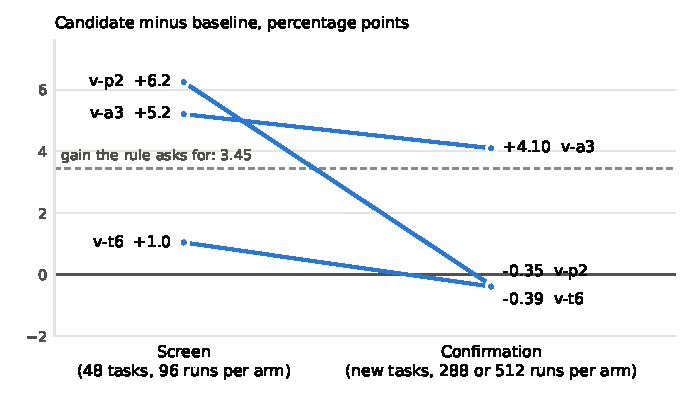
\includegraphics[width=0.72\linewidth]{fig/lead_gain.pdf}
\caption{Lead of each candidate in its screen on S against its gain in the confirmation run on other tasks, both in
percentage points against the baseline of the same block. The horizontal line is the gain that the pass rule asks
for.}
\label{fig:leadgain}
\end{figure}

The three candidates led their screens by $\LeadOne$, $\LeadTwo$ and $\LeadThree$ points. On new tasks their gains
were $\GainOne$, $\GainTwo$ and $\GainThree$ points (\cref{fig:leadgain}). Two leads vanished; the third candidate
kept most of its lead and still did not pass. We ask here, after the fact, what a lead on S is worth.

\paragraph{The noise of a screen.}
The baseline ran in all three screens, so each task of S has six baseline runs. The variation within tasks gives a
standard deviation of \ScreenSdArmRuns{} runs, or \ScreenSdArmPts{} points, for the total of one arm of 96 runs, and
\ScreenSdDiffPts{} points for the difference of two arms. S is a hard set for this model: \SNeverBase{} of its 48
tasks were solved in none of the six baseline runs, so the whole signal of a screen sits on 14 tasks.

\paragraph{The leader of equal arms.}
Suppose that no variant differs from the baseline, and that every arm total varies independently with the standard
deviation above. Then the best of five variants leads the baseline by \ScreenNullLeadFive{} points on average, and the
best of two by \ScreenNullLeadTwo{} points. A lead as large as the one observed, or larger, has probability
\ScreenNullPOne{} in the first screen (\ScreenLeadRunsOne{} runs, five variants), \ScreenNullPTwo{} in the second
(\ScreenLeadRunsTwo{} run, two variants) and \ScreenNullPThree{} in the third (\ScreenLeadRunsThree{} runs, two
variants). None of the three leads was unusual for a screen in which nothing differs.

That all five variants of the first screen were ahead looks stronger than it is. The five leads share one baseline
total, and that total, 19, is the lowest of the three baseline sessions on S (19, 21, 20). A low draw of the shared
baseline lifts every lead at once.

This calculation is a normal approximation with a noise estimate from six runs per task, and it assumes that a
variant has the same run-to-run noise as the baseline. We give it as a guide for planning, not as a test.

\paragraph{Consequences for the procedure.}
A screen of this size selects a candidate; it does not measure one. The leader's lead has to be discounted by the
selection effect before any plan is built on it, and the first two confirmations show what can remain of it. To rank
variants, the standard deviation of a difference would have to fall from \ScreenSdDiffPts{} points to about one
point, which needs roughly nine times the runs: about 830 runs per arm on tasks like those of S. That is larger than
a confirmation block. We conclude that the screen should be kept small and cheap, as a filter for broken builds and
a tie-break among variants, and that the number of confirmations, not the number of screens, limits what can be
learned.

\paragraph{The third candidate.}
In its confirmation the third candidate solved \ConfCandThree{} runs against \ConfBaseThree{} for the baseline. By
task, it was ahead on \CandThreeTasksUp{} tasks, behind on \CandThreeTasksDown{} and level on
\CandThreeTasksSame{}. The difference of \CandThreeDiffRuns{} runs is \CandThreeNoiseRatio{} standard deviations of
the run-to-run noise of a difference on H (\cref{sec:small}). Against the baseline session of the second
confirmation, which solved \RepeatHFirst{} runs on the same tasks, the difference is \CandThreeDiffEarlier{} runs, or
\CandThreeNoiseRatioEarlier{} standard deviations.

These ratios are post hoc, and they answer a narrower question than the rule does. Run-to-run noise asks whether the
same tasks, run again, would give the same difference. The rule asks whether the gain would hold on other tasks and
repositories, and its test, with repositories as clusters, gives $p = \GatePThree$, above the registered level. The
registered verdict stands: not confirmed. We do not call the third candidate an improvement. H has now been used for
two confirmations, and the third candidate was built after the result of the first of them was known. A further test
of this candidate needs tasks that no experiment has touched.

\subsection{Recomputation from the released rows}

The three confirmation blocks are in \texttt{runs.csv} with the rest. \Cref{sec:app-recheck} recomputes every
quantity of the three decisions from these rows with the released kit and compares it with the frozen reports;
all \RecheckQuantities{} quantities agree. The $p$-values of the first two applications are equal to four decimals,
\GatePOne{} and \GatePTwo{}. The recomputation confirms that this is a coincidence of two different data sets, with
63 against 62 solved runs of 288 in one and 103 against 101 of 512 in the other, and not a copying error.
